% Author: Alfredo Sánchez Alberca (email:asalber@ceu.es)
% Plot with the interquartile range
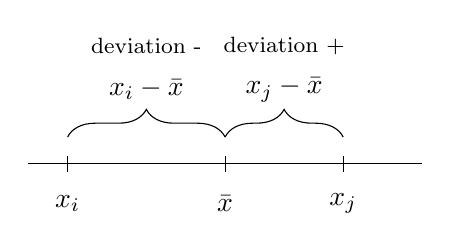
\begin{tikzpicture}[every label/.style={text=color1}]
\draw (0,1) -- (5,1);
\draw (2.5,0.9) -- (2.5,1.1);
\node at (2.5,0.5) {$\bar x$};
\draw (0.5,0.9) -- (0.5,1.1);
\node at (0.5,0.5) {$x_i$}; 
\draw (4,0.9) -- (4,1.1);
\node at (4,0.5) {$x_j$};  
\draw [decorate,decoration={brace,amplitude=10pt},yshift=4pt] (0.5,1.2) -- (2.5,1.2) node
[black,midway,yshift=0.6cm] {$x_i-\bar x$};
\draw [decorate,decoration={brace,amplitude=10pt},yshift=4pt] (2.5,1.2) -- (4,1.2) node
[black,midway,yshift=0.6cm] {$x_j-\bar x$};
\node at (1.5,2.5) {\footnotesize deviation -};
\node at (3.25,2.5) {\footnotesize deviation +};
\end{tikzpicture}